
\documentclass[11pt,a4paper]{article}
\usepackage[]{acl}
\usepackage{latexsym}
\usepackage{arydshln}
\usepackage{soul}

\renewcommand{\UrlFont}{\ttfamily\small}
\usepackage{microtype}




\usepackage{array}
\usepackage{pifont}
\usepackage{tabularx}
\usepackage{adjustbox}
\usepackage{multirow}
\usepackage{enumitem}
\usepackage{xspace}
\usepackage{tcolorbox}
\usepackage{booktabs,amsfonts,dcolumn}
\usepackage{url}
\usepackage{amsmath,amsthm,amsfonts,amssymb,bm,stmaryrd}
\usepackage[noorphans,vskip=0.75ex,leftmargin=2ex]{quoting}

\usepackage{amsmath}%
\usepackage{kantlipsum}
\usepackage{tabularx}
\usepackage[utf8]{inputenc} %
\usepackage[T1]{fontenc}    %
\usepackage{url}            %
\usepackage{booktabs,multirow}       %
\usepackage{amsfonts}       %
\usepackage{nicefrac}       %
\usepackage{microtype}      %


\usepackage{graphicx}
\usepackage{times}
\usepackage{epsfig}
\usepackage{graphicx}
\usepackage{amsmath}
\usepackage{amssymb}
\usepackage{xcolor,vwcol}
\usepackage{booktabs}
\newcommand\numberthis{\addtocounter{equation}{1}\tag{\theequation}}


\usepackage[OT6,T1]{fontenc}
\usepackage[utf8]{inputenc}
\usepackage[english]{babel}

\DeclareMathOperator{\E}{\mathbb{E}}

\usepackage{mathtools}
\DeclarePairedDelimiterX{\norm}[1]{\lVert}{\rVert}{#1}
\usepackage{multicol}
\usepackage[linesnumbered,ruled,vlined]{algorithm2e}
\usepackage{setspace}

\newcommand{\pushline}{\Indp}%
\newcommand{\popline}{\Indm\dosemic}%
\let\oldnl\nl%
\newcommand{\nonl}{\renewcommand{\nl}{\let\nl\oldnl}}%

\DeclareMathAlphabet{\pazocal}{OMS}{zplm}{m}{n} 
\usepackage{microtype}
\usepackage{graphicx}
\usepackage{colortbl}

\usepackage{booktabs} %
\usepackage{subcaption}
\usepackage{times}
\usepackage{latexsym}
\usepackage{makecell} 
\usepackage{amsfonts} 
\usepackage{amsmath} 
\usepackage{amssymb} 
\newcommand{\mC}[0]{\mathcal{C}}
\newcommand{\mCt}[0]{\mathcal{C}_T}
\newcommand{\mCv}[0]{\mathcal{C}_V}

\newcommand{\bridge}[1]{{\color{orange} \textbf{\textit{#1}}}}
\newcommand{\support}[1]{{\color{blue}\textit{#1}}}
\newcommand{\answer}[1]{{\color{green!55!black}\textbf{#1}}}
\newcommand{\sentid}[1]{{\color{green!55!black}#1}}
\newcommand{\armenian}{\fontencoding{OT6}\fontfamily{cmr}\selectfont}
\DeclareTextFontCommand{\textarmenian}{\armenian}


\newcommand\BibTeX{B\textsc{ib}\TeX}

\definecolor{brightmaroon}{rgb}{0.76, 0.23, 0.28}
\newcommand{\ac}[1]{{\textcolor{brightmaroon} {[#1 -- AC]}}}
\newcommand{\neww}[1]{{\color{black}{#1}}}
\renewcommand{\sectionautorefname}{\S}
\renewcommand{\subsectionautorefname}{\S}
\renewcommand{\subsubsectionautorefname}{\S}
\newcommand{\sect}{\S}
\newcommand{\red}[1]{\textcolor{black}{#1}}

\definecolor{cadmiumgreen}{rgb}{0.0, 0.42, 0.24}
\definecolor{burgundy}{rgb}{0.5, 0.0, 0.13}
\definecolor{darkviolet}{rgb}{0.58, 0.0, 0.83}
\definecolor{princetonorange}{rgb}{1.0, 0.56, 0.0}
\definecolor{darkmagenta}{rgb}{0.55, 0.0, 0.55}
\definecolor{cornellred}{rgb}{0.7, 0.11, 0.11}
	
\providecommand{\todo}[1]{
    {\protect\color{red}{[TODO: #1]}}
}

\providecommand{\danqi}[1]{
    {\protect\color{purple}{[Danqi: #1]}}
}

\providecommand{\jinhyuk}[1]{
    {\protect\color{blue}{[Jinhyuk: #1]}}
}

\providecommand{\alex}[1]{
    {\protect\color{teal}{[Alex: #1]}}
}

\providecommand{\todon}{
    {\protect\color{red}{00.00}}
}


\newcommand{\cmark}{\ding{51}}
\newcommand{\xmark}{\ding{55}}

\newcommand\sys[1]{\textsc{#1}}
\newcommand\ti[1]{\textit{#1}}
\newcommand\ts[1]{\textsc{#1}}
\newcommand\tf[1]{\textbf{#1}}
\newcommand\ttt[1]{\texttt{#1}}
\newcommand\mf[1]{\mathbf{#1}}
\newcommand\tmp[1]{\color{gray}{#1}}
\newcommand\warn[1]{\textbf{\color{red}{#1}}}
\newcommand\mr[1]{\mathrm{#1}}
\newcommand\mc[1]{\mathcal{#1}}
\newcommand{\cls}{\ttt{[CLS]}}
\newcommand{\tableindent}{~~}

\DeclareMathOperator*{\argmax}{arg\,max}
\DeclareMathOperator*{\argmin}{arg\,min}
\renewcommand{\paragraph}[1]{\vspace{0.2cm}\noindent\textbf{#1}}
\newcommand{\tpf}[1]{\noindent\textbf{#1}}


\newcommand{\ours}{DensePhrases}
\newcommand{\documentset}{\mathcal{D}}
\newcommand{\passageset}{\mathcal{P}}
\newcommand{\sentset}{\mathcal{S}}
\newcommand{\phraseset}{\mathcal{S}(\mathcal{D})}
\newcommand{\phraseinp}{\mathcal{S}(p)}
\newcommand{\wordset}{\mathcal{W}(\mathcal{D})}
\newcommand{\phrasedump}{\mf{H}}
\newcommand{\traincorpus}{\mathcal{C}}
\newcommand{\lm}{\mathcal{M}}

\DeclareSymbolFont{extraup}{U}{zavm}{m}{n}
\DeclareMathSymbol{\varheart}{\mathalpha}{extraup}{86}
\DeclareMathSymbol{\vardiamond}{\mathalpha}{extraup}{87}





\title{Long Context Question Answering via Supervised Contrastive Learning}

\author{Avi Caciularu$^{\clubsuit}\thanks{\;\; Work partly done as an intern at AI2.}$\hspace{1em}
\textbf{Ido Dagan$^\clubsuit$ \hspace{1em}Jacob Goldberger$^{\spadesuit}$ }\hspace{1em} Arman Cohan$^{\diamondsuit,\heartsuit}$\vspace{6pt}\\  
    $^\clubsuit$Computer Science Department, Bar-Ilan University, Ramat-Gan, Israel\\
    $^\spadesuit$Faculty of Engineering, Bar-Ilan University, Ramat-Gan, Israel\\
    $^\diamondsuit$Allen Institute for AI, Seattle, WA\\
    $^\heartsuit$Paul G. Allen School of Computer Science, University of Washington, Seattle, WA\\
    {\small\tt avi.c33@gmail.com, armanc@allenai.org} \\
    {\small\tt dagan@cs.biu.ac.il, jacob.goldberger@biu.ac.il }
}
\date{}

\begin{document}


\maketitle
	
\begin{abstract}

Continuous Integration (CI) is a software development practice that builds and tests software frequently (e.g., at every push). One main motivator to adopt CI is the potential to deliver software functionalities more quickly than not using CI. However, there is little empirical evidence to support that CI helps projects deliver software functionalities more quickly. Through the analysis of 162,653 pull requests (PRs) of 87 GitHub projects, we empirically study whether adopting a CI service (\textsc{TravisCI}) can quicken the time to deliver merged PRs. 
We complement our quantitative study by analyzing 450 survey responses from participants of 73 software projects.
Our results reveal that adopting a CI service may not necessarily quicken the delivery of merge PRs. Instead, the pivotal benefit of a CI service is to improve the decision making on PR submissions, without compromising the quality or overloading the project's reviewers and maintainers. The automation provided by CI and the boost in developers' confidence are key advantages of adopting a CI service. Furthermore, open-source projects planning to attract and retain developers should consider the use of a CI service in their project, since CI is perceived to lower the contribution barrier while making contributors feel more confident and engaged in the project.
		
\keywords{Continuous Integration \and Pull Request \and Delivery Time \and Code Review}
 
\end{abstract}


\section{Introduction}
\label{sec:intro}

% \begin{itemize}
%     \item Generic intro for deep speaker embeddings incl x-vectors
%     \item How are x-vectors used in speaker diar? AHC+PLDA, k-means, SC
%     \item How are x-vectors used in SV?
%     \item Reformulation as multiple tasks
%     \begin{itemize}
%             \item Although it works so well, current setup is single-task which transfer learns embeddings for unseen classes
%             \item By randomly sampling a subset of classes during training, we can easily formulate as multiple related tasks
%             \item Meta-learning generalizes across multiple tasks, hence a natural choice here
%     \end{itemize}
%     \item Contributions
%     \begin{itemize}
%         \item Generic speaker embeddings trained using meta-learning objectives, unlike prev works which focused on one
%         \item \textbf{(Pending results)} Application of relation networks for speaker embedding training (or) combining deep clustering with meta learning
%         \item Open-source toolkit for reproducible research
%     \end{itemize}
% \end{itemize}

Audio speaker embeddings refer to fixed-dimensional vector representations extracted from variable duration audio utterances and assumed to contain information relevant to speaker characteristics. In the last decade, speaker embeddings have emerged as the most common representations used for speaker-identity relevant tasks such as speaker diarization (speaker segmentation followed by clustering: \textit{who spoke when?}) \cite{anguera_DiarOverview2012} and speaker verification \textit{(does an utterance pair belong to same speaker?}) \cite{campbell_speakerRecogTutorial1997}.
Such applications are relevant across a variety of domains such as 
voice bio-metrics \cite{rahulamathavan_bioMetrics2019, scheffer_bioMetrics2013}, automated meeting analysis \cite{anguera2007acoustic,vanLeeuwen_meeting2006}, and clinical interaction analysis \cite{pal_clusterGAN2020, xiao2016technology}. Recent technology evaluation challenges \cite{ryant2019second, richey2018voices, Hansen_fearlessSteps2018, McLaren_SITW2016} have drawn attention to these domains by incorporating natural and simulated in-the-wild speech corpora exemplifying the many diverse technical facets that need to be addressed. 

While initial efforts toward training speaker embeddings had focused on generative modeling \cite{reynolds2000speaker,campbell_SVMGMM2006} and factor analysis \cite{dehak_ivectors2011}, deep neural network (DNN) representations extracted at bottleneck layers have become the standard choice in recent works. The most widely used representations are trained using a classification loss (d-vectors \cite{origdvec_variani2014deep}, x-vectors \cite{snyder_xvec2017, snyder_xvec2018}), while other training objectives such as triplet loss \cite{bredin_tristounet2017, zhang_triplet2018} and contrastive loss \cite{chung2018Voxceleb2} have also been explored.
%Following training, the output layer is removed and bottleneck representations are treated as speaker embeddings.
More recently, end-to-end training strategies \cite{Fujita2019, horiguchi2020endtoend, fujita2020endtoend} have been proposed for speaker diarization to address the mismatch between training objective (classification) and test setup (clustering, speaker selection, etc).

A common factor in the classification formulation is that all the speakers from training corpora are used throughout the training process for the purpose of loss computation and minimization. Typically, categorical cross-entropy is used as the loss function.
While the number of speakers (classes) can often be large in practice ($\mathcal{O}(10^3)$), the classification objective represents a single task, i.e., the same speaker set is used to minimize cross-entropy at every training minibatch.
This entails limited task diversity during the training process and offers scope for training better speaker-discriminative embeddings by introducing more tasks.
We note that a few approaches exist which introduce multiple objectives for embedding training, such as metric-learning with cross entropy \cite{XU2020394, ren2019} and speaker classification with domain adversarial learning \cite{zhou2019dann, wang2018dann}. While these approaches demonstrate improvements over a single training objective, the speaker set is often common across objectives (except in domain adversarial training where target speaker labels are assumed unavailable).
% \textbf{TO ADD: Check comments in source file}\\
% Contrast this work with multiple loss functions during training:
% 1. https://www.sciencedirect.com/science/article/pii/S092523122031016X
% 2. Combining CE with triplet: https://arxiv.org/pdf/1908.02283.pdf
% So-called multi-task frameworks esp in adversarial training: Here, mention that "task" in these works refers to the objective itself, like CE, triplet, etc
% 3. https://ieeexplore.ieee.org/stamp/stamp.jsp?tp=&arnumber=8683828 
% Check with Taejin about continual learning with replays for speaker embedding training

In this work we use the classification framework while training neural speaker embeddings, however we decompose the original classification task into multiple tasks wherein each training step optimizes on a new task. 
A common encoder is learnt over this ensemble of tasks and used for extracting speaker embeddings during inference.
At each step of speaker embedding training, we construct a new task by sampling speakers from the training corpus. For a large training speaker set available in typical training corpora,
generating speaker subsets results in a large number of tasks.
%sampling results in a factorially (right term?) large number of tasks. 
This provides a natural regularization to prevent task over-fitting. 
Our approach is inspired by the meta-learning \cite{Schmidhuber_thesis} paradigm, also known as {\it learning to learn}. Meta-learning optimizes at two-levels: within each task and across a distribution of tasks \cite{ravi2017}. This is in contrast to conventional supervised learning which optimizes a single task over a distribution of samples. 
In addition to benefits from increased task variability meta-learning has demonstrated success in unseen classes \cite{ravi2017, finn_maml2017,Andrychowicz_2016}.
This forms a natural fit for applications such as speaker diarization and speaker verification which often evaluate on speakers unseen during embedding training.

We compare our meta-learned models with x-vectors, which have established state-of-the-art performance in multiple applications \cite{snyder_xvec2017, snyder_xvec2018} including recent evaluation challenges such as DIHARD\cite{Sell2018_dihard} and VOiCES \cite{richey2018voices}. 
First, we develop a competitive wide-band x-vector baseline using the PyTorch toolkit (calibrated with identical performance with the Kaldi Voxceleb recipe\footnote{https://github.com/kaldi-asr/kaldi/tree/master/egs/voxceleb}). 
Next, we use two different metric-learning objectives to meta-learn the speaker embeddings: prototypical networks and relation networks. While both approaches share the task sampling strategy during the training phase, they differ in the choice of the comparison metric between samples. We evaluate our approaches on two different applications: speaker diarization and speaker verification to illustrate the generalized speaker discriminability nature of meta-learned embeddings. 
% Can expand on this after completing experiments?

The contributions of this work are as follows: we develop new speaker embeddings using meta-learning that are not restricted to an application.
Within each application, we demonstrate improvements using multiple corpora obtained under controlled as well as naturalistic speech interaction settings.
Furthermore, we identify conditions where meta-learning demonstrates benefits over conventional cross-entropy paradigm. 
We analyze diarization performance across different domains in the DIHARD corpora. We also consider the special case of impact of child age groups using internal child-adult interaction corpora from the Autism domain. We study the effect of data collection setups (near-field, far-field and obstructed microphones) and the level of degradation artifacts on the speaker verification performance.
While we present results using prototypical networks and relation networks, the proposed framework is independent of the specific metric-learning approach and hence offers scope for incorporating non-classification objectives such as clustering. It should be noted however that the application of relation networks has not been explored in speaker embedding research.
Finally, we present an open source implementation of our work, including x-vectors baselines, based on a generic machine learning toolkit (PyTorch)\footnote{https://github.com/manojpamk/pytorch\_xvectors}.










\section{Background}
\label{sec:background}

% \subsection{Meta-learning for speaker embeddings}

% \begin{itemize}
%     \item Includes protonets implementation “In defence of metric learning for speaker recognition” 
%     \item Talks about metric-learning (center loss?) “Comparison of metric-learning loss functions for E2E speaker verification” 
%     \item Protonets for short utterance speaker recognition 
%     \item \textbf{(Pending results)} Using deep clustering loss, based on spectral clustering: ||VVT - LLT||F 
% \end{itemize}

\subsection{Meta-Learning for Task Generalization}

Early works on meta-learning focused on adaptive learning strategies such as combining gradient descent with evolutionary algorithms \cite{yao_evolve1999,ABRAHAM20041}, learning gradient updates using a meta-network \cite{naik_metaNN1992} and using biologically inspired constraints for gradient descent \cite{bengio_synaptic1991, bengio1992optimization}.
Recent meta-learning approaches have addressed the issue of rapid generalization in deep learning, by learning to learn for a new task \cite{Andrychowicz_2016, finn_maml2017, ravi2017}.
This concept is inspired by the human ability to learn using a handful of examples. For instance children learn to recognize a new animal when presented with a few images as opposed to conventional DNNs which require thousands of samples for a new class.
The ability to quickly generalize to unseen classes is achieved by generating diversity in training tasks, for instance by using different sets of classes at each training step (see Fig. 1 in \cite{ravi2017}). Further, the classification setup (in terms of number of classes and samples per class) is controlled to match with that of the test task \cite{snell2017prototypical}.
Meta-learning has been successfully applied to achieve task generalization in computer vision \cite{ravi2017,snell2017prototypical,finn_maml2017} and more recently in natural language processing \cite{yu2018diverse,GaoH0S19, dou-etal-2019-investigating}.
Drawing parallels with the above applications, we train speaker embeddings with a large number of speaker classification tasks to improve over the conventional model which uses a single classification task. Since speaker sets differ between training steps, we replace the conventional softmax nonlinearity and cross-entropy loss combination with metric learning objectives used in previous meta-learning works \cite{snell2017prototypical,sung2018learning,vinyals2016matching,geng2019induction}.


\subsection{Meta-Learning Speaker Embeddings}

Few recent approaches have used a variant of meta-learning to train speaker embeddings, specifically the metric-learning objective from prototypical networks (protonets).
In \cite{chung2020defence}, the authors extend angular softmax objective to protonets and compare with various metric learning approaches for speaker verification. Across different architectures, angular prototypical loss outperforms other methods including conventional softmax objective. 
The authors in \cite{kye2020metalearning} applied protonets for short utterance speaker recognition and introduced global prototypes that mitigate the need for class sampling. 
In related applications, \cite{ko_protonets2020} and \cite{an2019shot} used protonets for small footprint speaker verification and few-shot speaker classification, respectively.
In \cite{wang_centroid2019}, the protonet loss was compared with triplet loss and evaluated on (open and close set) speaker ID and speaker verification tasks. 
However, previous approaches seldom compare embeddings trained using protonets with existing benchmarks based on x-vectors, except for \cite{ko_protonets2020} where a modified architecture was used owing to the nature of the task. Further, the class sampling strategy is not always used with protonets (e.g., \cite{chung2020defence,kye2020metalearning})
% triple-check above claim!)
which might inhibit task diversity during training. 
An exception from the above metric-learning approaches is \cite{kang2020domaininvariant}, where the authors train deep speaker embeddings using the model-agnostic meta-learning strategy to mitigate  domain mismatch for speaker verification.
To the best of our knowledge, meta-learning is yet to be applied for general-purpose speaker diarization, except for the specific case of dyadic speaker clustering in child-adult interactions in our recent work \cite{koluguri2020}. 

%> Protonets previously in speaker embedding applications
%> Connect relation networks to previous works, ones which learn the relation
% Refer to the Google Doc for a summary




\section{Question-Evidence Contrastive Loss}
\label{sec:method}
In this section, we elaborate on our novel proposed contrastive loss term, combining question-evidence similarity maximization (\sect\ref{subsec:qe_sim}), and question-type aware projections (\sect\ref{subsec:qt_aware}).

\subsection{Question-Evidence Similarity}
\label{subsec:qe_sim}
To encourage the long-context transformer model to capture relationships between the question and evidence sentences, we introduce an additional sequence-level loss that compares and contrasts the question with context sentences. 

The additional proposed loss $\mathcal{L}_{QE}$ is based on the InfoNCE loss~\cite{oord2018representation}, and is applied over instances consisting of triplet of vectors representing the question, an evidence sentence and distractor sentences. The loss encourages the question and evidence representations to become closer to each other, while pushing the question and distracting sentences away. 

Formally, the contrastive loss is defined as the sum of negative log-likelihood losses over all input examples, where each loss term discriminates the positive units from negative ones:
\begin{align}\label{eqn:loss}
    \mathcal{L}_{QE_i} = -\log \sum\limits_{s^+ \in \mathcal{S}^+_i} \left(\frac{e^{sim(s^+, q_i)/\tau_k}}{\sum\limits_{s \in \mathcal{S}_i} e^{sim(s, q_i)/\tau_k}}\right),
\end{align}
where $s$ ($q_i$) is the sentence (question) marker vector representation (see \texttt{$\langle$s$\rangle$} and \texttt{$\langle$/s$\rangle$} in Fig.~\ref{fig:model})%
, $\tau_k$ is the configurable temperature hyperparameter, and $sim(\cdot)$ is a similarity metric. $\mathcal{L}_{QE_i}$ serves a single example, and the final aggregated loss ${\mathcal{L}_{QE}}$ is obtained by averaging over all the examples.

We incorporate $\mathcal{L}_{QE}$ into the main QA span extraction/generation loss $\mathcal{L}_{QA}$ using the augmented loss:
\begin{equation*}
{\mathcal{L}=(1-\lambda)\cdot\mathcal{L}_{QA}+\lambda\cdot\mathcal{L}_{QE},}
\end{equation*}
where $\lambda$ is a weighting hyperparameter. 


The underlying $sim(\cdot)$ can take the form of a non-parametric similarity function, e.g., the dot product ($sim\left(s, q\right){=}s^\top q$) or the cosine similarity ($sim\left(s, q\right){=}\frac{s^\top q}{\norm{s}\norm{q}}$). However, we show empirically that using such similarity over the raw representations harms the performance results of the model, since seemingly, it is hard to find a shared representation that should optimize the two loss functions. Hence, we adopted linear projections, per question type, to cast the similarity learning objective into proxy linear spaces.




\subsection{Incorporating Question-Type Projections}
\label{subsec:qt_aware}
\red{Long-context QA benchmarks often provide a question-type label per instance as an additional challenge, such as ${\text{\{yes, no, span\}}}$ for HotpotQA. We hypothesize that maximizing question-evidence similarity under a question-type-specific sub-space can enable more flexibility and inductive bias to the model, for producing better representations and further improving the performance.}
Following \citet{iter-etal-2020-pretraining}, we define the following similarity function:
\begin{equation}
sim_k\left(s,q\right)=s^\top W_k q,
\label{eq:first_s}
\end{equation}
where $k$ is the expected question type and $W_k$ is the corresponding learnable projection matrix. Such linear projections ensure that a specific subspace per question type exists. We additionally incorporate different temperature hyperparameters $\tau_k$ per question type in Eq.~\ref{eqn:loss} (see the ablation in Table \ref{tab:ablations} for their effect). %
The dimensions of the proposed $W_k$ tend to be large, in accordance with the dimensions of the transformer's hidden-layers.\footnote{Empirically, we end up with $W_k\in\mathbb{R}^{768\times768}$ for base-sized models and $W_k\in\mathbb{R}^{1024 \times1024}$ for large-sized models.} Hence, following~\citet{barkan-etal-2020-within}, we apply new non-square linear projections instead of using $W_k$:
\begin{equation}
sim_k\left(s,q\right)=\frac{s_k^\top q_k}{\norm{s_k}\norm{q_k}},
\label{eq:cos_k}
\end{equation}
where we set $$s_k{:=}W^S_{k}s,\quad
q_k{:=}W^Q_{k}q,$$ and
$W^S_{k}$ (or $W^Q_{k}$) is the matrix that projects $s$ (or $q$) into a lower dimension, in the $k^\text{th}$ question-type sub-space. 
In order to improve the separation between the different sub-spaces induced by different question types, we generated additional negative instances per sentence, as follows. 

We projected every question-sentence pair using all the mappings according to the available question types, and computed their cosine similarity (according to Eq.~\ref{eq:cos_k}). Then, all the obtained scores were considered as negative, except the ones that belong to question-evidence pairs projected using the correct question-type mapping. %


\section{Experiments}
We conduct experiments on two ultra-fine entity typing datasets, {\bf \textsc{UFET}} (English) and {\bf \textsc{CFET}} (Chinese). Their data statistics are shown in Table \ref{tab:stat}. We mainly focus on and report the macro-averaged recall at the recall and expand stage, and concern mainly on the macro-$F1$ of the final prediction at the filter stage. We also evaluate the {\bf \textsc{\name}} models on the fine-grained (130 types) and coarse-grained (9 types) settings of entity typing without the recall and expand stage.
\subsection{UFET and CFET}
\subsubsection{Recall Stage}
\label{sec:recall}
We compare the recall@$K$ on the test sets of {\bf \textsc{UFET}} and {\bf\textsc{CFET}} between the trained MLC model (introduced in \ref{sec:mlc}) and a traditional BM25 model \cite{bm25} in Figure \ref{fig:recall}. The MLC model uses the RoBERTa-large as backbone and is tuned based on the recall@$128$ on the development set. We use AdamW optimizer with a learning rate of $2\times10^{-5}$. Results show that MLC is a strong recall model, it consistently has better recall compared to BM25 on both {\bf\textsc{UFET}} and {\bf\textsc{CFET}} dataset, and the recall@$128$ reaches over $85\%$ on {\bf \textsc{UFET}}, and over $94\%$ on {\bf \textsc{CFET}}.

\begin{figure}[t]
     \centering
     \begin{subfigure}[h]{0.5\textwidth}
         \centering
         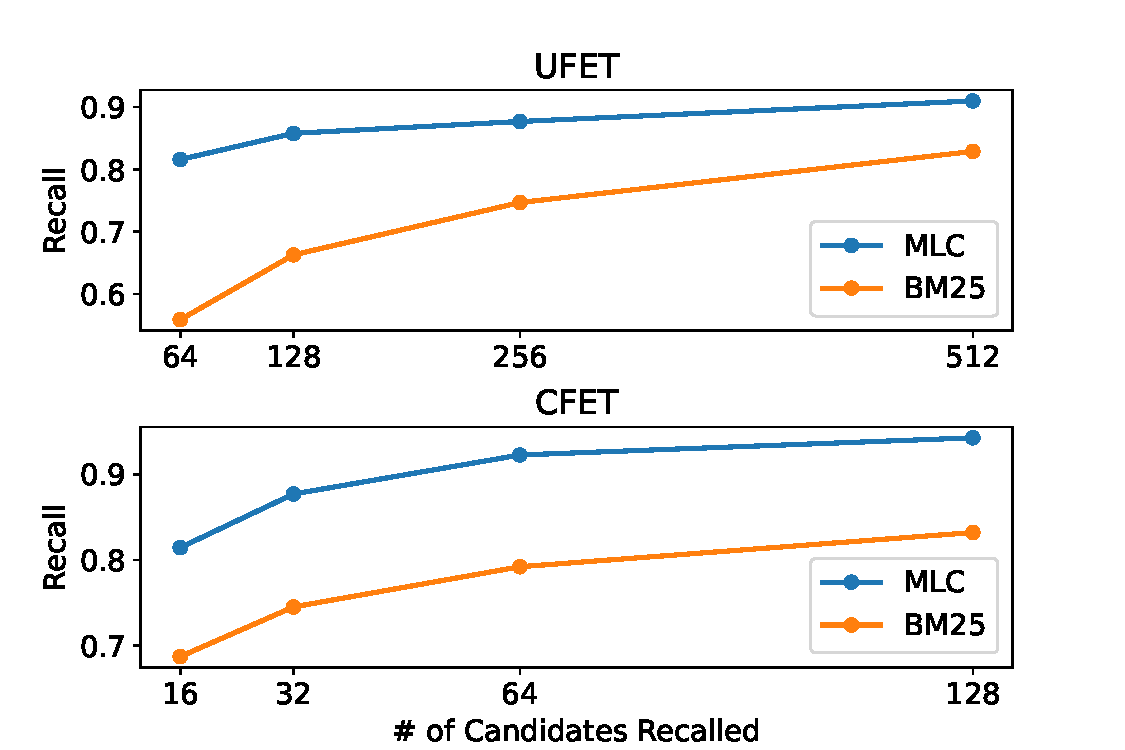
\includegraphics[width=\textwidth]{src/img/recall_compare_bm25.pdf}
         \label{fig:mb2}
     \end{subfigure}   
 \caption{Recall@$K$ of MLC and BM25.}
 \label{fig:recall}
\end{figure}

\subsection{Expand Stage}
\label{sec:expand}
In Table \ref{tab:expand}, we evaluate the F1 scores of all candidates expanded by exact match, and top-$10$ candidates expanded by the MLM using Bert-large. We also demonstrate the improvement of recall by using candidate expansion in Figure \ref{fig:expand_improvement}. On {\bf \textsc{UFET}} dataset, expanding around $32$ additional candidates based on $112$ MLC candidates results in $2\%$ higher recall compared to recalling all $128$ candidates by MLC. The recall of $128$ candidates after the expansion is comparable to the recall of $180$ candidates recalled from MLC. Similarly, expanding $10$ candidates is comparable to additionally recalling $80$ candidates using MLC.
In our experiments, we replace the last $48$ candidates recalled by MLC with the candidates recalled by MLM and Exact match for {\bf \textsc{UFET}} and $10$ for {\bf \textsc{CFET}}. We found the expand stage has a positive effect on the final performance of {\bf \textsc{\name}}s, and helps them reach SOTA performance (analyze in Sec. \ref{sec:analyze}).


\begin{table}[t]
\centering
\scalebox{0.75}{
\begin{tabular}{cccccc} 
\toprule
{\bf \textsc{Dataset}} & {\bf \textsc{Expand}} &   {\bf \textsc{P}}  & {\bf \textsc{R}}  &  {\bf \textsc{F1}} & \small{Avg \# Expanded}  \\ \midrule
\multirow{2}{*}{\bf \textsc{UFET}} & {\bf \textsc{Match}}      & 11.2   & 11.3     & 9.8    & 5.23     \\
      & {\bf \textsc{MLM}}  &  8.5     &   17.1   &  10.7  &    10    \\ \midrule
\multirow{2}{*}{\bf \textsc{CFET}} & {\bf \textsc{Match}}   &  11.4  &  14.5  & 11.2   & 4.57    \\
 & {\bf \textsc{MLM}}  & 21.3   &  19.5  & 17.7    & 10    \\ \midrule
\end{tabular}}
\caption{Evaluation of the recalled candidates.}
\label{tab:expand}
\end{table}
\begin{figure}[t]
     \centering
     \begin{subfigure}[h]{0.45\textwidth}
         \centering
         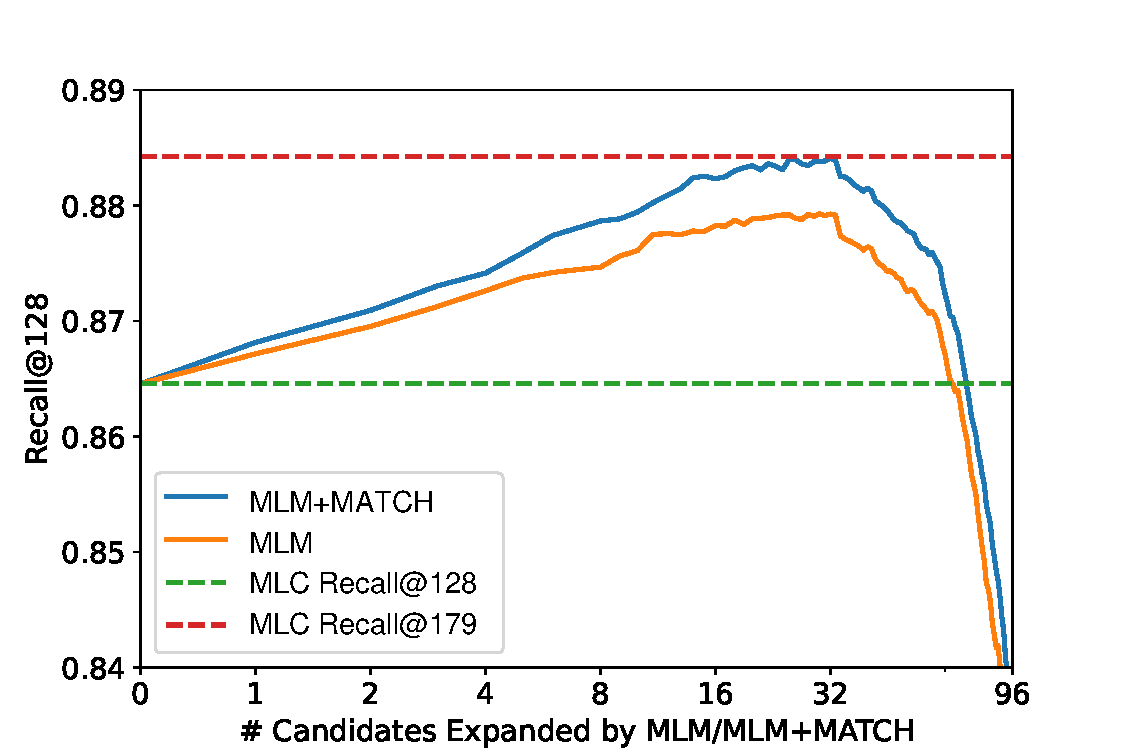
\includegraphics[width=\textwidth]{src/img/recall_ufet.pdf}
         \caption{Recall@$128$ on {\bf \textsc{UFET}} by including different number of expanded candidates. }
         \label{fig:c1}
     \end{subfigure}
     \vfill
     \begin{subfigure}[h]{0.45\textwidth}
         \centering
         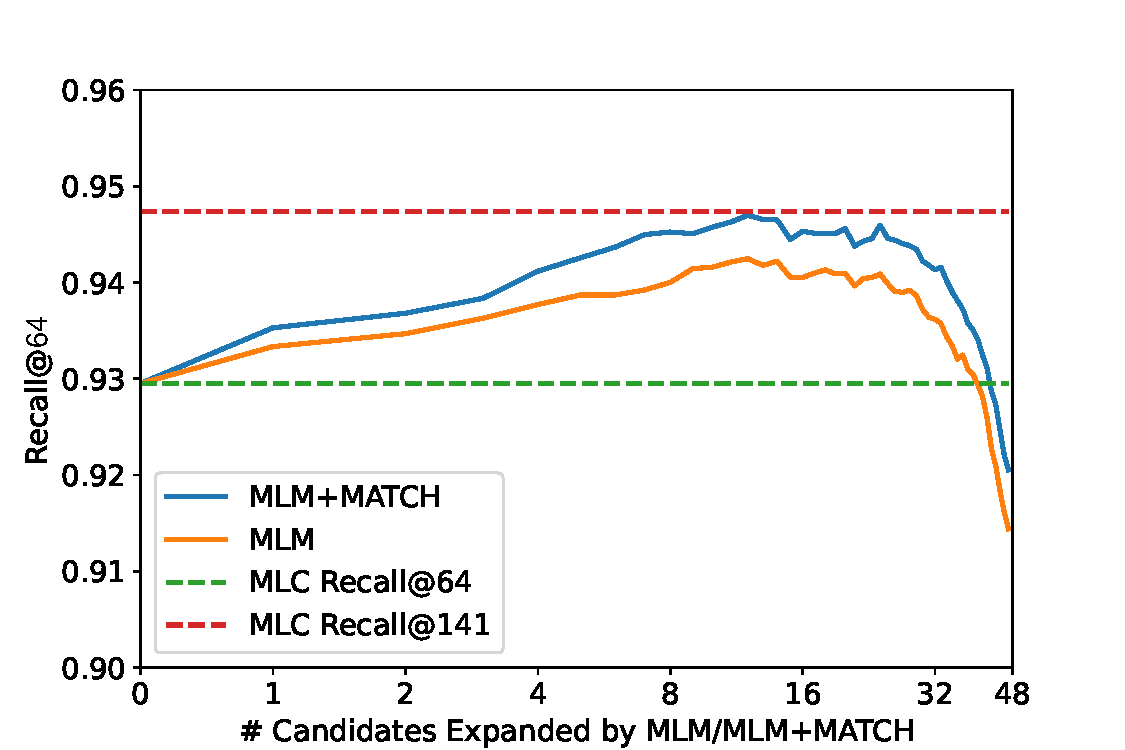
\includegraphics[width=\textwidth]{src/img/recall_cfet.pdf}
         \caption{Recall@$64$ on {\bf \textsc{CFET}} by including different number of expanded candidates.}
         \label{fig:c2}
     \end{subfigure}
\caption{Demonstration of the effect of expand stage. $x$-axis represents the number of candidates expanded by MLM/MLM+MATCH among these $128$ candidates. }
\label{fig:expand_improvement}
\end{figure}
\label{sec:exp_expand}
\subsection{Filter Stage and Final Results.}
\begin{table}[h!]
\centering
\scalebox{0.73}{
\renewcommand{\arraystretch}{1}
\begin{tabular}{cllll} \toprule
\multicolumn{2}{l}{\bf \textit{Base Models on UFET} }     & \bf \textsc{P}    & \bf \textsc{R}   & \bf \textsc{F1}  \\ \midrule
\multicolumn{5}{l}{\emph{MLC-like models}}        \\
\color{blue} \bf \texttt{B}& {\bf \textsc{Box4Types}}\cite{box4types}  & 52.8 & 38.8 & 44.8  \\
\color{blue}\bf \texttt{B}& {\bf \textsc{LDET}}$^\dagger$  \cite{onoe-durrett-2019-learning}          & 51.5 & 33.0 & 40.1 \\ 
\color{blue}\bf \texttt{B}& {\bf \textsc{MLMET}}$^\dagger$   {\cite{mlmet}}   & 53.6 & 45.3 & 49.1  \\
\color{blue}\bf \texttt{B}& {\bf \textsc{PL}}  \cite{ding2021prompt}   & 57.8 & 40.7 & 47.7 \\
\color{blue}\bf \texttt{B}& {\bf \textsc{DFET}}    \cite{dfet}      & 55.6 & 44.7 & 49.5 \\
\color{blue}\bf \texttt{B}& {\bf \textsc{MLC}} (reimplemented by us) & 46.5 & 34.9 & 39.9 \\ 
\color{red}\bf \texttt{R}& {\bf \textsc{MLC}} (reimplemented by us) & 42.2 & 44.9 & 43.5 \\ \hline 
\multicolumn{5}{l}{\emph{Seq2seq based models}}      \\
\color{blue}\bf \texttt{B} & {\bf \textsc{LRN} }  {\cite{liu-etal-2021-fine}}              & 54.5 & 38.9 & 45.4  \\\hline
\multicolumn{5}{l}{\emph{Filter models under our recall-expand-filter paradigm}}      \\
\color{blue}\bf \texttt{B} & {\bf \textsc{Vanilla CE}$_{128}$}   & 47.2 & 48.5 & 47.8 \\ 
\color{blue}\bf \texttt{B} & {\bf \textsc{\name-S$_{128}$}} (Ours)  & 53.2 & 48.3 & {\bf 50.6} \\ 
\color{blue}\bf \texttt{B} & {\bf \textsc{\name-S$_{128}$ w/o C2C}}   (Ours)   & 52.3 & 48.3 & 50.2 \\ 
\color{blue}\bf \texttt{B} & {\bf \textsc{\name-B$_{128}$}} (Ours)    & 49.9 & 50.0 & 49.9 \\ 
\color{blue}\bf \texttt{B} & {\bf \textsc{\name-B$_{128}$ w/o C2C}} (Ours)     & 49.9 & 48.2 & 49.0 \\ \hline
\color{red}\bf \texttt{R} & {\bf \textsc{Vanilla CE}$_{128}$}   & 49.6 & 49.0 & 49.3 \\ 
\color{red}\bf \texttt{R} & {\bf \textsc{\name-S$_{128}$}} (Ours)  & 53.3 & 47.3 & 50.1 \\ 
\color{red}\bf \texttt{R} & {\bf \textsc{\name-S$_{128}$ w/o C2C}}   (Ours)  & 53.2 & 46.6 & 49.7 \\ 
\color{red}\bf \texttt{R} & {\bf \textsc{\name-B$_{128}$}} (Ours)  & 52.5 & 47.9 & 50.1 \\ 
\color{red}\bf \texttt{R} & {\bf \textsc{\name-B$_{128}$ w/o C2C}} (Ours)     & 52.7 & 46.4 & 49.3 \\ \hline
\midrule
\multicolumn{2}{l}{\bf \textit{Large Models on UFET} }     & \bf \textsc{P}    & \bf \textsc{R}   & \bf \textsc{F1}  \\ \midrule
\multicolumn{5}{l}{\emph{MLC-like models}}        \\
\color{red}\bf \texttt{R} & {\bf \textsc{MLC}}  \cite{npcrf}               & 47.8 & 40.4 & 43.8  \\
\color{red}\bf \texttt{R} & {\bf \textsc{MLC-NPCRF}} \cite{npcrf}             & 48.7 & 45.5 & 47.0  \\
\color{red}\bf \texttt{R} & {\bf \textsc{MLC-GCN}} \cite{xiong-etal-2019-imposing}     & 51.2 & 41.0 & 45.5 \\
\color{blue}\bf \texttt{B} & {\bf \textsc{PL}}  \cite{ding2021prompt}       & 59.3 & 42.6 & 49.6  \\
\color{blue}\bf \texttt{B} & {\bf \textsc{PL-NPCRF}}  \cite{npcrf}  & 55.3 & 46.7 & {50.6}\\ \hline
\multicolumn{4}{l}{\emph{Cross-encoder based models and {\bf \textsc{\name}}s}}      \\
\color{red}\bf \texttt{R} & {\bf \textsc{LITE+L}}  \cite{lite}             & 48.7 & 45.8 & 47.2  \\
\color{teal}\bf \texttt{RM} & {\bf \textsc{LITE+NLI+L}} \cite{lite} & 52.4 & 48.9 & {50.6} \\ \hline
\multicolumn{4}{l}{\emph{Filter models under our recall-expand-filter paradigm}}   \\ 
\color{blue}\bf \texttt{B} & {\bf \textsc{Vanilla CE$_{128}$}}   & 50.3 & 49.6 & 49.9 \\ 
\color{blue}\bf \texttt{B} & {\bf \textsc{\name-S$_{128}$}}  (Ours)   & 52.5 & 49.1 & 50.8 \\ 
\color{blue}\bf \texttt{B} & {\bf \textsc{\name-S$_{128}$ w/o C2C}}   (Ours)   & 54.1 & 47.1 & 50.4 \\ 
\color{blue}\bf \texttt{B} & {\bf \textsc{\name-B$_{128}$}} (Ours)    & 54.0 & 48.6 & 51.2 \\ 
\color{blue}\bf \texttt{B} & {\bf \textsc{\name-B$_{128}$ w/o C2C}} (Ours)     & 52.8 & 48.3 & 50.4 \\ \hline
\color{red}\bf \texttt{R} & {\bf \textsc{Vanilla CE$_{128}$}}   & 54.5 & 49.3 & 51.8 \\ 
\color{red}\bf \texttt{R} & {\bf \textsc{\name-S$_{128}$}}  (Ours)   & 50.8 & 49.8  &  50.3 \\ 
\color{red}\bf \texttt{R} & {\bf \textsc{\name-S$_{128}$ w/o C2C}}   (Ours)   & 51.5 & 48.8 & 50.1 \\ 
\color{red}\bf \texttt{R} & {\bf \textsc{\name-B$_{128}$}} (Ours)    & 51.9 & 50.8 & 51.4 \\ 
\color{red}\bf \texttt{R} & {\bf \textsc{\name-B$_{128}$ w/o C2C}} (Ours)     & 51.6 & 51.6 & 51.6 \\ \hline
\color{teal}\bf \texttt{RM} & {\bf \textsc{\name-B$_{128}$ w/o C2C}} (Ours) & 56.3 & 48.5 & {\bf 52.1} \\ \hline
\midrule
\end{tabular}}
\caption{Macro-averaged UFET result. {\bf \textsc{LITE+L}} is LITE without NLI pretraining, {\bf \textsc{LITE+L+NLI}} is the full LITE model. Methods marked by $\dagger$ utilize either distantly supervised or augmented data for training. {\bf \textsc{\name-S$_{128}$}} denotes we use $128$ candidates recalled and expanded from the first two stages.}
\label{tab:ufet}
\end{table}
\begin{table}[t]
\centering
\scalebox{0.75}{
\renewcommand{\arraystretch}{1}
\begin{tabular}{cllll} \toprule
\multicolumn{2}{l}{\bf \textit{Models on CFET} }     & \bf \textsc{P}    & \bf \textsc{R}   & \bf \textsc{F1}  \\ \midrule
\multicolumn{5}{l}{\emph{MLC-like models}}        \\
\color{purple}\bf \texttt{N}& {\bf \textsc{MLC}} & 55.8 & 58.6 & 57.1 \\  
\color{purple}\bf \texttt{N}& {\bf \textsc{MLC-NPCRF}} \cite{npcrf}     & 57.0 & 60.5 & 58.7 \\ 
\color{purple}\bf \texttt{N}& {\bf \textsc{MLC-GCN}} \cite{xiong-etal-2019-imposing}   & 51.6 & 63.2 & 56.8 \\ 
\color{brown}\bf \texttt{C}& {\bf \textsc{MLC}} & 54.0 & 59.5 & 56.6 \\  
\color{brown}\bf \texttt{C}& {\bf \textsc{MLC-NPCRF}} \cite{npcrf}   & 54.0 & 61.6 & 57.3 \\  
\color{brown}\bf \texttt{C}& {\bf \textsc{MLC-GCN}} \cite{xiong-etal-2019-imposing} & 56.4 & 58.6 & 57.5 \\ \midrule 
\multicolumn{5}{l}{\emph{Filter models under our recall-expand-filter paradigm}}      \\
\color{purple}\bf \texttt{N} & {\bf \textsc{Vanilla CE}}   & 57.6 & 64.3 & 60.7 \\ 
\color{brown}\bf \texttt{C} & {\bf \textsc{Vanilla CE}}   & 54.0 & 63.3 & 58.3 \\  \hline
\color{purple}\bf \texttt{N} & {\bf \textsc{\name-S$_{64}$}} (Ours)  & 58.4 & 62.1 & 60.2 \\ 
\color{purple}\bf \texttt{N} & {\bf \textsc{\name-S$_{64}$ w/o C2C}}   (Ours)   & 59.1 & 61.5 & 60.3 \\ 
\color{purple}\bf \texttt{N} & {\bf \textsc{\name-B$_{64}$}} (Ours)    & 56.7 & 66.1 & 61.1 \\ 
\color{purple}\bf \texttt{N} & {\bf \textsc{\name-B$_{64}$ w/o C2C}} (Ours)     & 58.8 & 64.1 & 61.4 \\ \hline
\color{brown}\bf \texttt{C} & {\bf \textsc{\name-S$_{64}$}} (Ours)  & 55.5 & 62.6 & 58.8 \\ 
\color{brown}\bf \texttt{C} & {\bf \textsc{\name-S$_{64}$ w/o C2C}}   (Ours)   & 54.0 & 63.4 & 58.3 \\ 
\color{brown}\bf \texttt{C} & {\bf \textsc{\name-B$_{64}$}} (Ours)    & 55.0 & 63.5 & 59.0 \\ 
\color{brown}\bf \texttt{C} & {\bf \textsc{\name-B$_{64}$ w/o C2C}} (Ours)     & 57.3 & 61.3 & 59.3 \\ \hline
\midrule
\end{tabular}}
\caption{Macro-averaged CFET result.}
\label{tab:cfet}
\end{table}

In this section, we report the performance of {\bf \textsc{MCCE}} variants as the filter models and compare them with various strong baselines that we will introduce later. We also compare the inference speed of different models in this section. For filter models, we treat the number of candidates $K$ recalled and expanded by the first two stages as hyper-parameters, and tune it on the development set. We found the choice of PLM backbones has a non-negligible effect on the performance, and the PLM backbone of previous methods varies. Therefore for fairer comparisons to baselines, we conduct experiments of {\bf \textsc{\name}} using different backbone PLMs for our {\bf \textsc{\name}} models and report the results. For all {\bf \textsc{\name}} models, we use AdamW optimizer with a learning rate tuned between $5\times 10^{-6}$ and $2\times 10^{-5}$. The batch size we use is $4$ and we train the models for at most $50$ epochs with early stopping. {\bf \textsc{UFET}} also provides a large dataset obtained from distant supervision such as entity linking, we do not use it and only train and evaluate our models on human-labeled data.
\paragraph{Baselines}
The {\bf \textsc{MLC}} model we used for the recall stage and the cross-encoder ({\bf \textsc{CE}}) we introduced in Sec. \ref{sec:vanilla_ce} are natural baselines. We also compare our methods with recent PLM-based methods. {\bf \textsc{LDET} }\cite{onoe-durrett-2019-learning} is an MLC with Bert-base-uncased and ELMo \cite{elmo} trained on 727k examples automatically denoised from the distantly labeled UFET. {\bf \textsc{GCN} }\cite{xiong-etal-2019-imposing} uses GCN to model type correlations and obtain type embeddings. Types are scored by dot-product of mention and type embeddings. The original paper uses BiLSTM as the mention encoder and we use the results re-implemented by \citet{npcrf} using RoBERTa-large. {\bf \textsc{Box4Type} }\cite{box4types} uses Bert-large as the backbone and uses box embedding to encode mentions and types for training and inference. {\bf \textsc{LRN} }\cite{liu-etal-2021-fine} use Bert-base as the encoder and an LSTM decoder to generate types in a seq2seq manner. {\bf \textsc{MLMET} }\cite{mlmet} is a {\bf \textsc{MLC}} with Bert-base, but first pretrained by the distantly-labeled data augmented by masked word prediction, then finetuned and self-trained on the 2k human-annotated data. {\bf \textsc{PL}} \cite{ding2021prompt} uses prompt learning for entity typing. {\bf \textsc{DFET} }\cite{dfet} uses {\bf \textsc{PL}} as backbone and is a multi-round automatic denoising method for 2k labeled data. {\bf \textsc{LITE} }\cite{lite} is the previous SOTA system that formulates entity typing as textual inference. {\bf \textsc{LITE}} uses RoBERTa-large-MNLI as the backbone, and is a cross-encoder (introduced in Sec. \ref{sec:vanilla_ce}) with designed templates and a hierarchical loss. \citet{npcrf} proposes {\bf \textsc{NPCRF}} to enhance backbones such as {\bf \textsc{PL}} and {\bf \textsc{MLC}} by modeling type correlations, and reach performance comparable to {\bf \textsc{LITE}}.

\paragraph{Naming Conventions}
Let {\bf \textsc{\name-S}} be the {\bf \textsc{\name}} model that treats candidates as sub-tokens, and {\bf \textsc{\name-B}} be the model representing candidates as fixed-size blocks. The {\bf \textsc{\name}} model without {\bf \textsc{C2C}} attention (mentioned in Sec. \ref{sec:attn}) is denoted as {\bf \textsc{\name-B} w/o C2C}. For PLM backbones used in {\bf \textsc{UFET}}, we use {\color{blue} \bf \texttt{B}}, {\color{red} \bf \texttt{R}}, {\color{teal} \bf \texttt{RM}} to denote BERT-base-cased \cite{bert}, RoBERTa \cite{liu2019roberta}, and RoBERTa-MNLI \cite{liu2019roberta} respectively. For {\bf \textsc{CFET}}, we adopt two widely-used Chinese PLM, BERT-base-Chinese and NeZha-base-Chinese, and denote them as {\color{brown} \bf \texttt{C}} and {\color{purple} \bf \texttt{N}} respectively. 

\paragraph{UFET Results} We show the results of {\bf \textsc{UFET}} dataset in Table \ref{tab:ufet}. The results show that: (1) The recall-expand-filter paradigm is effective. Filter models outperform all baselines without the paradigm by a large margin. The vanilla CE under our paradigm reaches $51.8$ F1 compared to more complexed CE {\bf \textsc{LITE}} with $50.6$ F1 (2) {\bf \textsc{\name}} models reach SOTA performances. {\bf \textsc{\name-S$_{128}$}} with BERT-base performs best and reaches {\bf 50.6} F1 score, which is comparable to previous SOTA performance of large models such as {\bf \textsc{LITE+NLI+L}} and {\bf \textsc{PL+NPCRF}}. Among large models, {\bf \textsc{\name-B$_{128}$ w/o C2C}} also reaches SOTA performance with {\bf 52.1} F1 score. (3) {\bf \textsc{C2C}} attention is not necessary on large models, but is useful in base models. (4) Large models can utilize type semantics better. We found {\bf \textsc{\name-B}} outperforms {\bf \textsc{\name-S}} on large models, but underperforms {\bf \textsc{\name-S}} on base models. (5) Backbone PLM matters. We found the performance of {\bf \textsc{Vannila CE}} under our paradigm is largely affected by the PLM it used. It reaches $47.8$ F1 with BERT-base and $51.8$ F1 with RoBERTa-large. For {\bf \textsc{\name}} models, we found {\bf \textsc{\name}} performs better than {\bf \textsc{\name-B}} with BERT, and worse than {\bf \textsc{\name-B}} with RoBERTa. 

\begin{table*}[t]
\centering
\scalebox{0.9}{
\begin{tabular}{lllcc} \toprule
\bf \textsc{Model}  & \bf \textsc{\# FP} & \bf \textsc{Attn} & \bf \textsc{sents/sec} & \bf \textsc{F1} \\ \midrule
{\bf \textsc{MLC}} & \small{$1$}  & \small{$L_S^2D$} & 58.8 & 43.8\\
{\bf \textsc{LITE+NLI+L (CE)}}  & \small{$N$}  & \small{$L_S^2D$} & 0.02 & 50.6\\ \midrule \hline
\multicolumn{5}{l}{\emph{filter stage inference speed.}}  \\
{\bf \textsc{Vanilla CE$_{128}$}}  & \small{$128$}  & \small{$L_S^2D$} & 1.64 & 51.8 \\ 
{\bf \textsc{\name-S$_{128}$}}  & \small{$1$}  & \small{$(L_S+128)^2D$} & 60.8 & 50.1 \\ 
{\bf \textsc{\name-B$_{128}$}}  & \small{$1$}  & \small{$(L_S+128B)^2D$} & 22.3 & 51.4\\ 
{\bf \textsc{\name-B$_{128}$ w/o C2C}}  & \small{$1$}  & \small{$(L_S^2+256L_S B + 128 B^2)D$} & 25.2 & {\bf 52.1}\\ \bottomrule
\end{tabular}}
\caption{Inference speed comparison of models. {\bf \textsc{\# FP}} means the number of PLM forward passes required by a single inference. {\bf \textsc{ATTN}} column lists the theoretical attention complexity.  We also report the practical inference speed {\bf \textsc{sents/sec}} and the {\bf \textsc{F1}} scores on {\bf \textsc{UFET}} with RoBERTa-large architecture.}
\label{tab:speed}
\end{table*}

\begin{table}[t]
\centering
\scalebox{0.85}{
\renewcommand{\arraystretch}{1}
\begin{tabular}{cllll} \toprule
\multicolumn{2}{l}{\bf \textit{Models} }     & \bf \textsc{P}    & \bf \textsc{R}   & \bf \textsc{F1}  \\ \midrule
\multicolumn{5}{l}{\emph{coarse (9 types) Open Entity}}        \\ \hline
\color{red}\bf \texttt{R} & {\bf \textsc{MLC}}   & 76.8 & 78.5 & 77.6 \\ 
\color{red}\bf \texttt{R} & {\bf \textsc{Vanilla CE$_{9}$}}   & 82.3 & 81.0 & 81.6 \\ 
\color{red}\bf \texttt{R} & {\bf \textsc{\name-S$_{9}$}}   & 77.0 & 87.7 & 82.0 \\ 
\color{red}\bf \texttt{R} & {\bf \textsc{\name-B$_{9}$ w/o C2C}}   & 77.2 & 85.4 & 81.1 \\ \hline
\multicolumn{5}{l}{\emph{fine (130 types)}}        \\ \hline
\color{red}\bf \texttt{R} & {\bf \textsc{MLC}}   & 70.4 & 63.7 & 66.9  \\ 
\color{red}\bf \texttt{R} & {\bf \textsc{Vanilla CE}$_{130}$}   & 67.9 & 66.4 & 67.1 \\ 
\color{red}\bf \texttt{R} & {\bf \textsc{\name-S$_{130}$}}   & 65.8 & 71.8 & 68.7 \\ 
\color{red}\bf \texttt{R} & {\bf \textsc{\name-B$_{130}$ w/o C2C}}   & 64.1 & 70.5 & 67.1 \\ \hline
\midrule
\end{tabular}}
\caption{Micro-averaged results on UFET fine and coarse.}
\label{tab:ufet-coarse-fine}
\end{table}

\paragraph{CFET Results} We conduct experiments on {\bf \textsc{CFET}} and compare {\bf \textsc{\name}} models with several strong baselines:  {\bf \textsc{NPCRF}} and {\bf \textsc{GCN}} with MLC-like architecture, and {\bf \textsc{Vanilla CE}} under out paradigm which is proved to be better than {\bf \textsc{LITE}} on {\bf \textsc{UFET}}. The results are shown in Table \ref{tab:cfet}. Similar to results in {\bf \textsc{UFET}}, filter models under our paradigm significantly outperform MLC-like baselines, $+2.0$ F1 for Nezha-base and $+1.8$ F1 for BERT-base-Chinese. In {\bf \textsc{CFET}}, {\bf \textsc{\name}-B} is significantly better than {\bf \textsc{\name}-S}, on both Nezha-base and BERT-base-Chinese, indicating the importance of type semantics in Chinese language. We also find that {\bf \textsc{\name} w/o C2C} is generally better than  {\bf \textsc{\name} w/ C2C}, it is possibly because the C2C attention distracts the candidates from attending to mention and contexts.
\paragraph{Speed Comparison} Table \ref{tab:speed} shows the theoretical inference complexity (number of PLM forward passes, and attention complexity), and practical inference speed (number of sentences inferred per second) of different models. We conduct the speed test using NVIDIA TITAN RTX for all models, and the inference batch size is 4.
At the filter stage, the inference speed of {\bf \textsc{\name-S}} is on par with {\bf \textsc{MLC}} (even slightly faster because we don't need to score all types), and is about 40 times faster than {\bf \textsc{Vannila CE}} and thousands of times faster than {\bf \textsc{LITE}}. {\bf \textsc{\name-B w/o C2C}} is not significantly faster than {\bf \textsc{\name-B}} as expected. It's possibly because the computation related to the block attention is not fully optimized by existing deep learning frameworks. The speed advantage of {\bf \textsc{\name-B w/o C2C}} over {\bf \textsc{\name-B}} will be greater with more candidates.


\subsection{Fine-grained and Coarse-grained Entity Typing}
We also conduct experiments on Fine-grained (130-class) and Coarse-grained (9-class, also known as ``Open Entity'') entity typing, and the results are shown in Table \ref{tab:ufet-coarse-fine}. As the type candidate set is much smaller in these settings, we skip the recall and expand stages and directly run the filter models and compare them to baselines. Results show that both {\bf \textsc{\name}-S} and {\bf \textsc{\name}-B} are still better than {\bf \textsc{MLC}} and {\bf \textsc{Vanilla CE}}, and {\bf \textsc{\name}-S} is better than {\bf \textsc{\name}-B} on coarser-grained cases possibly because the coarser-grained types are simpler in surface-forms and {\bf \textsc{\name}-S} will not lose many type semantics.






\section{Conclusion}
In this work, we proposed an effective sequence-level contrastive loss for improving the performance of long-range transformers in solving QA tasks that require reasoning over long contexts. We demonstrate consistent improvement when using our approach on three different models over two different benchmarks.
For future work, we propose exploring variations of our proposed supervised loss on other long-context tasks, such as long-document and multi-document summarization, and integrating our method into information retrieval re-ranker models.

\section*{Acknowledgement}
This work is partially supported by NSF grant No.1910100, Amazon research award, DARPA No. HR00111990074. We thank the anonymous reviewers for their insightful comments.
\section*{Ethical Considerations}
Our work in understanding the role of maximizing the similarity between question and evidence pairs. Therefore, there is a limited risk associated with the quality of annotated evidence sentences in the dataset, as there is no guarantee that our model will always
generate non-biased and factual content. Therefore, caution must
be exercised when the model is deployed in practical settings, where the evidence quality is vague and cannot be verified.


\bibliography{acl2021,anthology}
\bibliographystyle{acl_natbib}
\clearpage
\appendix
\section*{Appendix}

\section{Question-Evidence Similarity Demonstration}
\label{sec:appndx1}

In this section, we further interpret the outcome of our contrastive loss.

We apply PCA over the relevant normalized token representations of the validation data of HotpotQA (i.e., the question and answers representations in Fig.~\ref{fig:model}), and depicted them in~\ref{fig:pca}. The projected representations of the correct and wrong answers are equally distributed at the beginning of the training (left figure). After several epochs when the model converged (right figure), the answer representations' manifold got closer to the questions' representations (in terms of radial distance). Each beam in the figure corresponds to a different question type (there are 3 in HotpotQA). The correct evidence representations (green dots) are the closest among the whole answer representations, confirming that our additional contrastive loss term generalizes and maximizes the question-evidence similarity. 


\section{Datasets and Finetuning Details}
\label{sec:appndx2}
In this section, we provide details, regrading finetuning and hyper-parameter configuration, over the benchmarks we used during our experiments.

\subsection{QAsper}
\label{subsec:qasper}
Since some of the questions included in QAsper are not answerable, we apply our contrastive loss only over examples that are answerable and contain at least one evidence sentence. 

We train all models using the Adam optimizer~\citep{kingma2014adam} and a triangular learning rate scheduler \cite{howard2018universal} with 10\% warmup. To determine number of epochs, peak learning rate, and batch size, we performed manual hyperparameter search on a subset of the training data. We searched over \{1, 3, 5\} epochs with learning rates \{$1e^{-5}$, $3e^{-5}$, $5e^{-5}$, $9e^{-5}$\}, and found that smaller batch sizes generally work better than larger ones. Our final configuration was 10 epochs, peak learning rate of $5e^{-5}$, and batch size of 2, which we used for all reported experimental settings.  When handling full text, we use gradient checkpointing~\cite{gradckpt} to reduce memory consumption. We run our experiments on a single RTX 8000 GPU, and each experiment takes 30--60 minutes per epoch. 


\subsection{HotpotQA}
\label{subsec:hotpotqa}
We used the HotpotQA-distractor dataset~\cite{yang-etal-2018-hotpotqa}. Each example in the dataset is includes a question and 10 paragraphs from different documents, extracted from Wikipedia. Two gold paragraphs include the relevant information for properly answering the question, mixed and shuffled with eight distractor paragraphs (for the full dataset statistics, see~\citet{yang-etal-2018-hotpotqa}). There are two goals for this task: detecting the supporting facts, i.e., evidence sentences, as well as extraction of the correct answer span. 

For preparing the data for training and evaluation, we follow the same finetuning scheme of the CDLM~\cite{caciularu-etal-2021-cdlm-cross} and the Longformer~\cite{longformer}; For each example, we concatenate the question and all the 10 paragraphs in one long context. We particularly use the following input format with special tokens and our document separators: ``\texttt{[CLS] [q] question [/q] $\langle$\texttt{doc-s}$\rangle$$\langle$t$\rangle$ $\texttt{title}_{\texttt{1}}$ $\langle$/t$\rangle$} \texttt{$\langle$s$\rangle$} $\texttt{sent}_{\texttt{1,1}}$ \texttt{$\langle$/s$\rangle$} \texttt{$\langle$s$\rangle$} $\texttt{sent}_{\texttt{1,2}}$ \texttt{$\langle$/s$\rangle$} $\langle$\texttt{/doc-s}$\rangle$ \texttt{...} \texttt{$\langle$t$\rangle$ $\langle$\texttt{doc-s}$\rangle$ $\texttt{title}_{\texttt{2}}$ $\langle$/t$\rangle$ }  $\texttt{sent}_{\texttt{2,1}}$ \texttt{$\langle$/s$\rangle$} \texttt{$\langle$s$\rangle$} $\texttt{sent}_{\texttt{2,2}}$ \texttt{$\langle$/s$\rangle$} \texttt{$\langle$s$\rangle$} \texttt{...}'' where \texttt{[q]}, \texttt{[/q]}, $\langle$\texttt{t}$\rangle$, $\langle$\texttt{/t}$\rangle$, \texttt{$\langle$s$\rangle$}, \texttt{$\langle$/s$\rangle$}, \texttt{[p]} are special tokens representing, question start and end, paragraph title start and end, and sentence start and end, respectively. The new special tokens were added to the models vocabulary and randomly initialized before task finetuning. We use global attention to question tokens, paragraph title start tokens as well as sentence tokens. 
The model's structure is taken from ~\citet{longformer}.

As in~\citet{longformer,caciularu-etal-2021-cdlm-cross}, we finetune our models for 5 epochs, using a batch size of 32, learning rate of $1e^{-4}$, 100 warmup steps. Finetuning on our models took $\sim$6 hours per epoch, using four 48GB RTX8000 GPUs for finetuning our models. For generating the CDLM-large results, we pretrined our version using the code from \url{https://github.com/aviclu/CDLM/tree/main/pretraining}.


\begin{figure*}
\centering
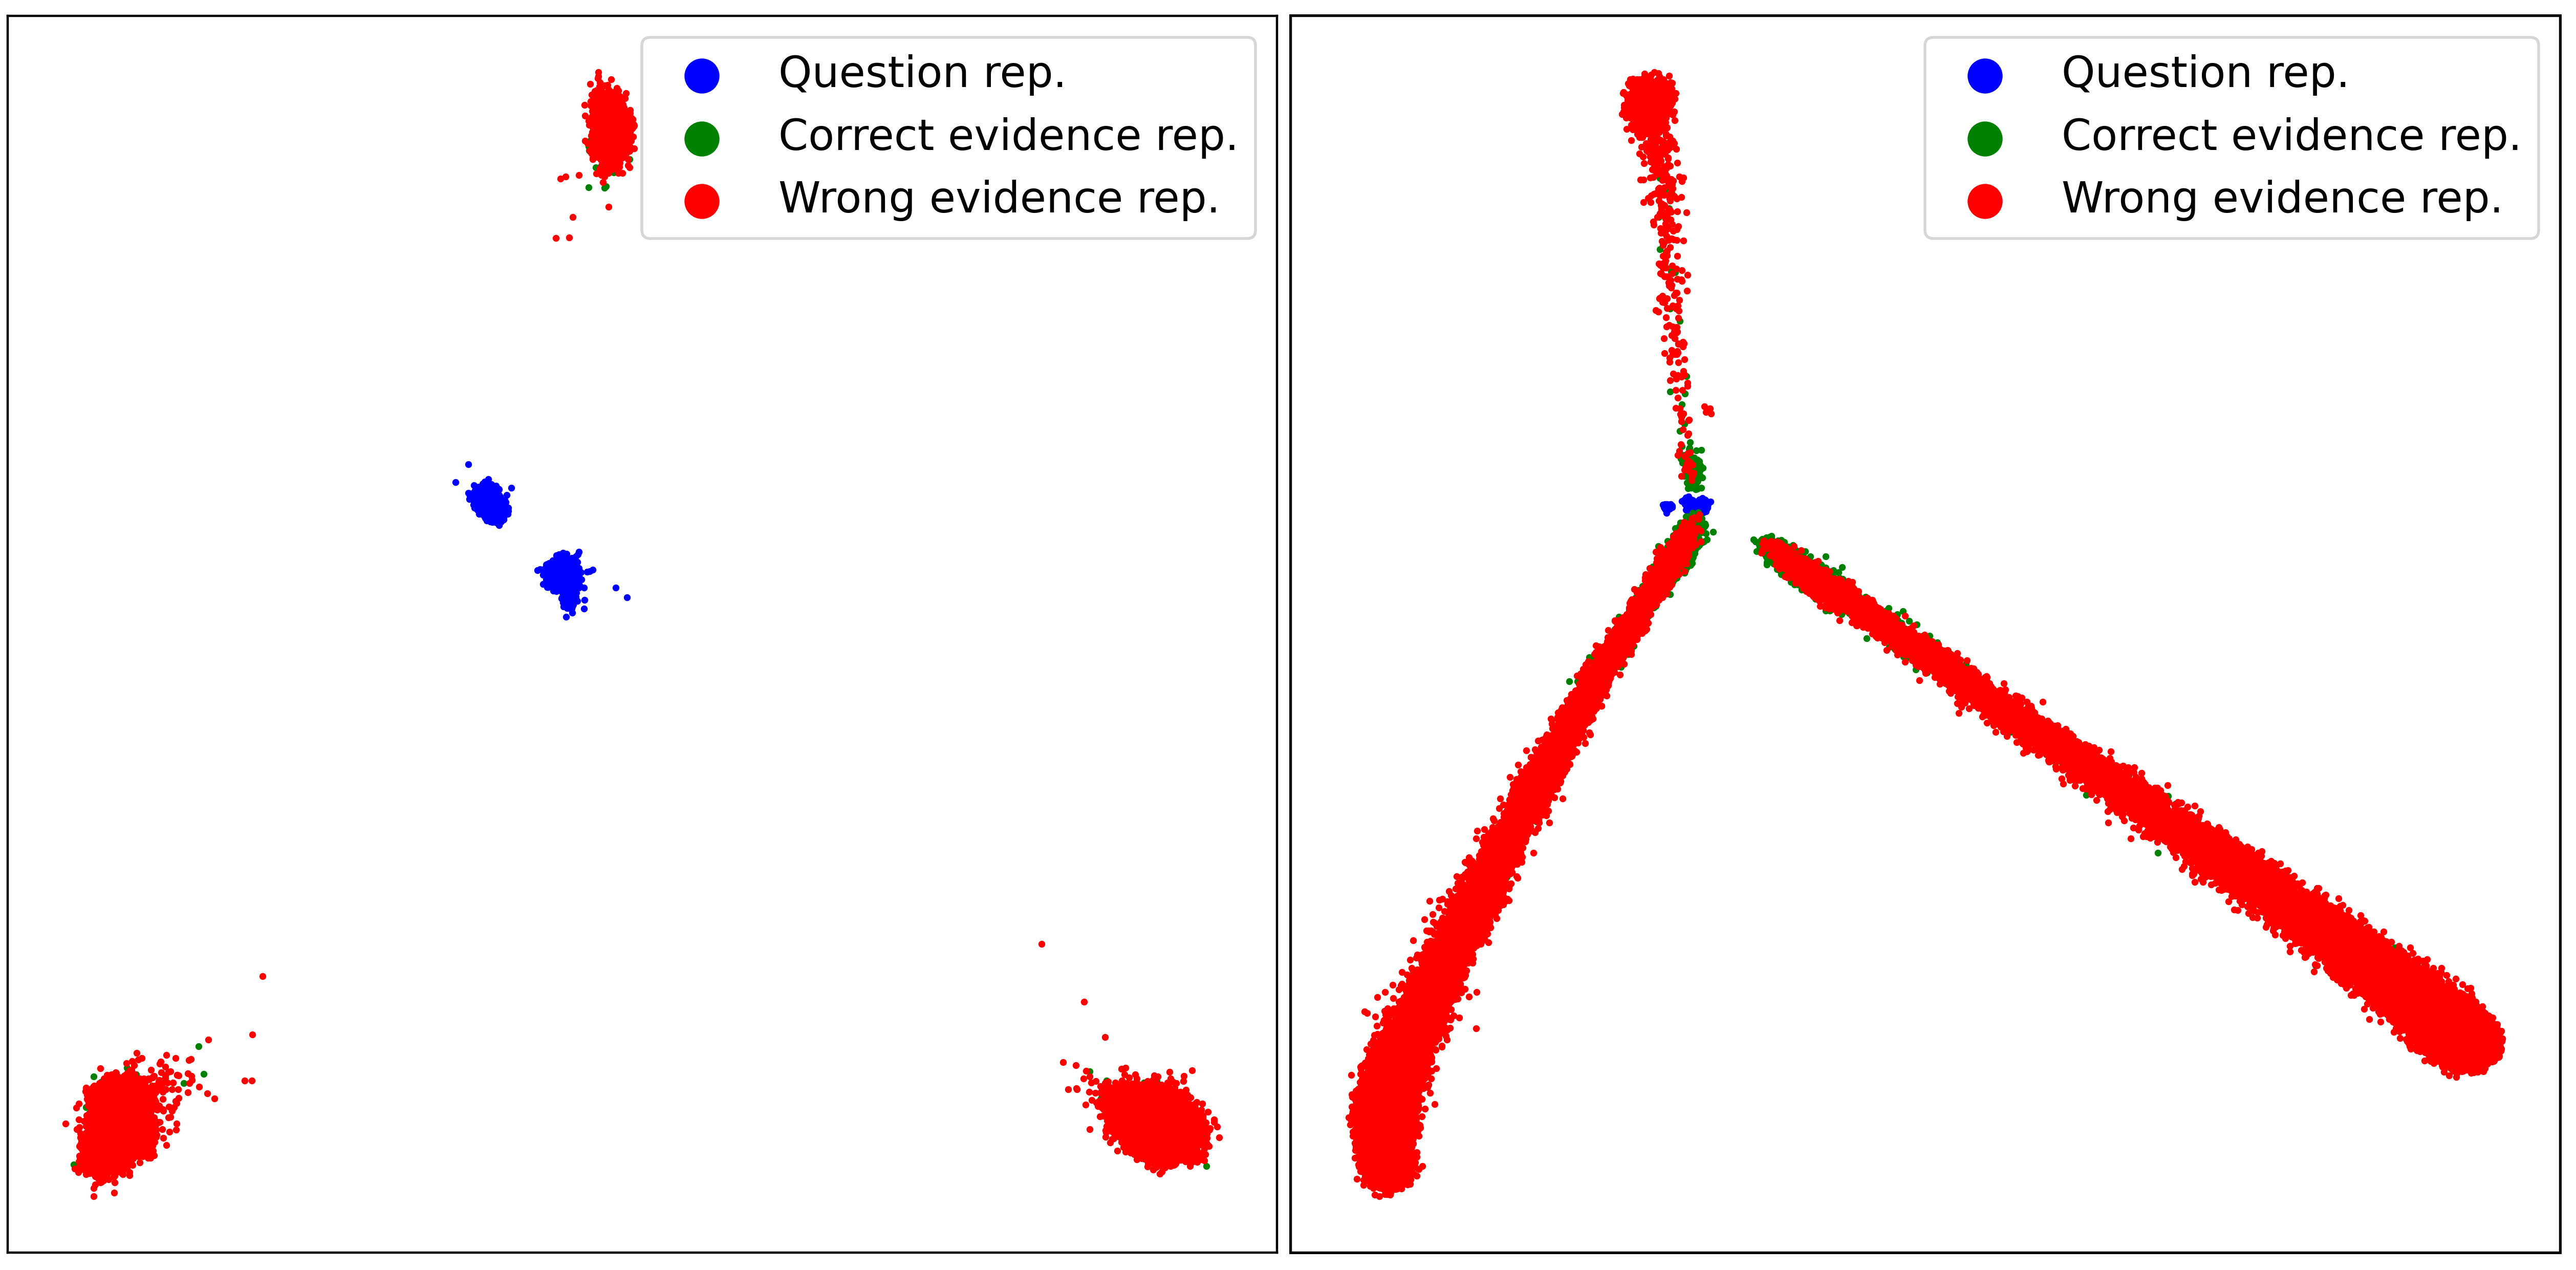
\includegraphics[width=.98\linewidth]{figures/pca_figures_3.png}
  \caption{PCA plots of the learned question and answer token embeddings on the HotpotQA validation set, comparing early training epochs results (left) and results after model convergence (right). The wrong evidence representations correspond to both wrong evidences, or correct evidences using the wrong question type projections (our soft negatives).}
  \label{fig:pca}
\end{figure*}


\section{Contrastive Loss Details}
\label{sec:contrastive}
In this section, we provide the details for reproducing our contrastive term, which is relevant for both QAsper and HotpotQA.

We searched over $d\times\{d,\frac{d}{2},\frac{d}{4},\frac{d}{8}\}$ to determine the linear projections' dimensions, where $d$ is the model's hidden layer representation dimension (it depends on the size of the model). In order to determine the temperature hyperparameter $\tau$, we searched over $\{0.2,0.4,0.6,0.8,1.0\}$ per question type (if applicable). We also applied dropout with a rate of ${p=0.1}$ over the linear projections, which consistently improved the results over all the benchmarks. Finally, we searched for the best performing $\lambda$ hyperparameter over the values of $\{0.2,0.4,0.6,0.8,1.0\}$.



\end{document}
